% English version. Build: pdflatex main_en -> bibtex main_en -> pdflatex main_en x2
% Figures in report/figures_en/ come from: python scripts/make_figures.py --lang en

\documentclass[11pt]{article}
\usepackage{acl}
\usepackage{times}
\usepackage{latexsym}
\usepackage[T5,T1]{fontenc}
\usepackage[utf8]{inputenc}
\usepackage{microtype}
\usepackage{graphicx}
\usepackage{booktabs}
\usepackage{amsmath}
\usepackage{amssymb}
\usepackage{multirow}
\usepackage{tikz}
\usetikzlibrary{arrows.meta, positioning, fit, backgrounds}

\makeatletter
\renewcommand\paragraph{\@startsection{paragraph}{4}{\z@}%
  {1.2ex \@plus1ex \@minus.2ex}{-1em}{\normalfont\normalsize\bfseries}}
\makeatother
\setcounter{topnumber}{2}
\renewcommand{\topfraction}{0.9}
\renewcommand{\textfraction}{0.07}
\renewcommand{\floatpagefraction}{0.75}

\graphicspath{{figures_en/}}

\title{Re-evaluating CIRAG on Vietnamese Multi-hop QA:\\
       A Refusal-Based Stopping Test and an Evidence-Based Replacement}

\author{
  Tan Nguyen Dang Duy, Huy Tran Anh, Tien Le Van, and Tram Nguyen Hong \\
  \textit{Faculty of Information Technology} \\
  \textit{University of Science, VNU-HCM} \\
  Ho Chi Minh City, Vietnam \\
  \texttt{\{25C1502208, 25C1100780, 25C1106995, 25C1107056\}@student.hcmus.edu.vn}
}

\begin{document}
\maketitle

\begin{abstract}
CIRAG \citep{wei2026cirag} compresses retrieved passages into $(s,r,o)$ triples to reduce noise,
and its authors report a large gain over earlier iterative retrieval methods. We reimplement
the method and test it on the dataset and backbone used in the original paper, reproducing
the reported margin to within 0.6 EM points. On ViMQA \citep{le2022vimqa}, a Vietnamese
multi-hop QA dataset, this margin does not appear. Four controlled experiments show that the
cause lies neither in our code, the Vietnamese prompts, a broken pipeline stage, nor backbone
capability. Instead, the cause is the method's stopping test. ACMG widens the context only
when the model itself says it cannot answer, so it trusts the model's judgement rather than
checking the context. As the backbone becomes stronger, it says this less often. The system
therefore almost always stops at the narrowest context level and answers wrongly from there.
We replace this test with one that checks the evidence itself. The new test requires the core
triple set to span as many documents as a multi-hop question needs, and it raises EM from
50.80 to 60.40 with no extra model calls.
\end{abstract}

\section{Introduction}
\label{sec:intro}

Retrieval-augmented generation \citep{lewis2020rag} works well on simple questions but
struggles with multi-hop reasoning because a single retrieval pass cannot gather pieces of
evidence that only make sense together. Iterative retrieval \citep{trivedi2023ircot} addresses
this problem by dividing the search into several rounds. Each round uses what the system has
just learned to form the next query. More recent work uses triples rather than passages as
the unit of retrieval \citep{fang2024trace, fang2025kirag}, which narrows the evidence and
reduces noise.

CIRAG \citep{wei2026cirag} addresses two separate problems in this line of work. The first is
greedy single-path expansion. Earlier methods keep only the single best triple at each step,
so an early mistake affects later steps, while the parallel evidence branches needed for
complex questions are lost. The second problem is a mismatch between the detail provided by
the evidence and the detail the question needs. Triples are clean and low-noise but lack
context, while passages provide full context with more noise. Thus, no fixed level suits
every question.

To limit greedy expansion, CIRAG proposes the ICI retrieval module (Iterative
Construction-Integration), based on the Construction-Integration model from cognitive
psychology \citep{kintsch1978ci}. The construction stage collects every triple from the
newly retrieved passages and ranks them to form a broad candidate pool. The integration
stage gives this pool and the reasoning history to the backbone model. The model selects
the triples that the question needs, called the core triple set, and writes the query for
the next round. Because the model can select several triples at once, the core set can
include evidence from several reasoning branches rather than only one.

To address the level-of-detail problem, CIRAG proposes the ACMG generation module (Adaptive
Cascaded Multi-Granularity Knowledge-Enhanced Generation). At each level, the system gives
the model the context from that level and asks it to answer. If the context is insufficient,
the model must return a fixed refusal string instead of guessing. The module begins at the
triple level and moves to sentences and then passages only after it receives a refusal.

We reimplement CIRAG and evaluate it on ViMQA \citep{le2022vimqa}, a Vietnamese multi-hop
QA dataset. On the original paper's dataset, our code reproduces its reported gain, but this
gain does not appear on ViMQA. The rest of this report investigates why. We make four
contributions:

\begin{itemize}
  \itemsep0.1em
  \item A verified reimplementation. We run it on 2WikiMultihopQA with the original
        backbone, and the margin over IRCoT it measures sits within 0.6 EM points of the one
        the paper reports (\S\ref{sec:results}).
  \item CIRAG relies on the model's refusal to tell whether the context is enough. That
        signal is wrong in both directions: the model refuses even when the evidence is
        already there, and answers even when it is missing (\S\ref{sec:analysis}).
  \item A replacement stopping test that asks the core triple set to span at least two
        documents instead of waiting for the model to refuse. It lifts EM from 50.80 to
        60.40 at no extra model calls (\S\ref{sec:fix}).
  \item Four explanations for why CIRAG's margin does not appear on ViMQA, each ruled out by
        an experiment that changes exactly one variable (\S\ref{sec:ruleout}).
\end{itemize}

\section{Related Work}
\label{sec:related}

\paragraph{Text-based iterative retrieval.} IRCoT \citep{trivedi2023ircot} alternates
between writing a reasoning step and retrieving evidence, using the sentence it has just
written as the next query. Self-Ask \citep{press2023selfask} divides a question into explicit
sub-questions. Because each round adds a whole passage to the context, noise increases over
successive rounds.

\paragraph{Triple-based iterative retrieval.} To reduce this noise, one line of work uses
triples instead of passages as the retrieval unit. HippoRAG \citep{jimenez2024hipporag} builds
a knowledge graph from extracted triples, while KiRAG \citep{fang2025kirag} extends a chain
of triples round by round. However, these methods keep only the best triple at each step and
fix the representation at the triple level.

CIRAG differs from both lines of work in exactly these two ways. It keeps a set of core
triples rather than a single chain, and it widens the context in stages rather than using a
fixed level.

\section{Method}
\label{sec:method}

CIRAG runs two modules in sequence (Figure~\ref{fig:pipeline}). ICI retrieves and filters
evidence into a core triple set, and ACMG produces the answer from that set. The original
paper includes a third module, Trajectory Distillation, which trains a small model to copy
the reasoning steps of a large model and thus reduce cost. We do not implement this module,
so every result in this report is compared with the paper's \emph{w/o TD} setting.

\begin{figure*}[t]
\centering
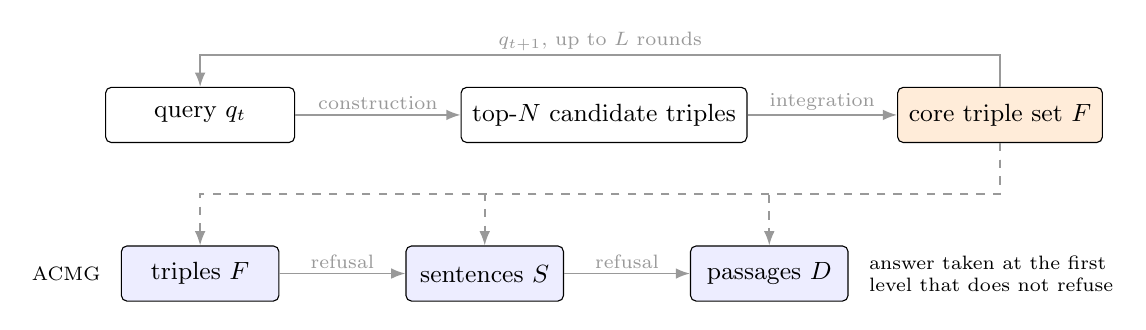
\begin{tikzpicture}[
  font=\small,
  b/.style={draw, rounded corners=2pt, align=center, inner sep=4pt, minimum height=7mm},
  lv/.style={b, fill=blue!7, minimum width=20mm},
  ar/.style={-{Latex[length=1.8mm]}, gray!80, line width=0.6pt},
  lb/.style={font=\scriptsize, inner sep=1.5pt},
]
% -- ICI: vong lap giua hai giai doan --
\node[b, minimum width=24mm]                       (q)    {query $q_t$};
\node[b, right=21mm of q, minimum width=32mm]      (cand) {top-$N$ candidate triples};
\node[b, right=19mm of cand, minimum width=26mm, fill=orange!15] (f) {core triple set $F$};

\draw[ar] (q)    -- node[lb, above] {construction} (cand);
\draw[ar] (cand) -- node[lb, above] {integration} (f);
\draw[ar] (f.north) -- ++(0,4mm) -| node[lb, pos=0.25, above] {$q_{t+1}$, up to $L$ rounds} (q.north);

% -- ACMG: cascade noi tiep, leo thang khi bi tu choi --
\node[lv, below=13mm of q]    (t)  {triples $F$};
\node[lv, right=16mm of t]    (se) {sentences $S$};
\node[lv, right=16mm of se]   (d)  {passages $D$};

\draw[ar] (t)  -- node[lb, above] {refusal} (se);
\draw[ar] (se) -- node[lb, above] {refusal} (d);

% F sinh ra ca ba muc
\draw[ar, dashed] (f.south) -- ++(0,-6.5mm) -| (t.north);
\draw[ar, dashed] (f.south) -- ++(0,-6.5mm) -| (se.north);
\draw[ar, dashed] (f.south) -- ++(0,-6.5mm) -| (d.north);
\node[lb, right=2mm of d, align=left] {answer taken at the first\\level that does not refuse};
\node[lb, left=2mm of t, align=right] {ACMG};
\end{tikzpicture}
\caption{The CIRAG pipeline. ICI alternates between the construction and integration stages to
build the core triple set $F$. ACMG first tries to answer from $F$ and only moves to sentences
and then passages when the model returns a refusal. The dashed arrows show that all three
levels derive from $F$, so a gap left by the integration stage carries into all three
(\S\ref{sec:limit-empty}).}
\label{fig:pipeline}
\end{figure*}

\paragraph{ICI.} Each round has two stages. The construction stage retrieves the top-$K$
passages for query $q_t$, collects their triples, and reranks them to select the top-$N$
candidates. The integration stage gives the candidate pool and the history $H_{<t}$ to the
backbone model. The model keeps the core triple set $F_t$ and writes the next query $q_{t+1}$.
The loop stops when the model emits \texttt{<no question>}, after at most $L$ rounds.

Each triple records its source sentence and passage. Two reverse maps, written $M^S$ and
$M^D$, turn $F$ into the sentence set $S = M^S(F)$ and the passage set $D = M^D(F)$. The
three sets $F$, $S$, $D$ are the context levels used by ACMG.

\paragraph{ACMG.} The system offers $F$, then $S$, then $D$ to the model and asks for an
answer, following the order triples $\prec$ sentences $\prec$ passages. If the context is
not enough, the model must return a fixed refusal string. The first level that is not
refused becomes the answer:
\begin{equation}
\label{eq:acmg}
g^\star = \min_{\prec}\{g \in G : \mathrm{Suf}(a^{(g)}) = 1\},\quad a^\star = a^{(g^\star)}
\end{equation}
where $\mathrm{Suf}(a)$ is true when $a$ does not match the refusal template. If no level
qualifies, the system falls back to the passage-level answer. Both the $\mathrm{Suf}$ test
and the fact that $S$ and $D$ derive from $F$ are the source of the problems in
\S\ref{sec:analysis}.

\section{Data}
\label{sec:data}

ViMQA \citep{le2022vimqa} is a Vietnamese multi-hop QA dataset written by hand from
Vietnamese Wikipedia articles and based on the HotpotQA layout
\citep{yang2018hotpotqa}. Each question includes ten passages. Two contain the evidence,
while eight act as distractors. The dataset also provides labels that mark the sentence
containing the evidence.

We randomly sample 500 questions from the validation split. If each question searched only
its own ten passages, the system would almost always find both evidence passages, making
retrieval unimportant. Following IRCoT, we merge the passages from all questions and remove
duplicates by title, producing a shared corpus of 1,969 passages. The system must then find
two evidence passages among nearly two thousand rather than among ten.

\section{Experimental Setup}
\label{sec:setup}

The hyperparameters follow the original paper ($K{=}10$, $N{=}30$, $L{=}4$). We replace two
components to support Vietnamese. First, we use the Vietnamese\_Embedding model, which
achieves recall@10 of 0.920 on the 1,969-passage corpus. Second, we rewrite the triple
extraction prompt in Vietnamese, producing 22,697 triples for the full corpus. The reasoning
model is Gemini 2.5 Flash, while triple extraction uses the cheaper Flash Lite because this
stage is easier and accounts for most calls.

\paragraph{Metrics.} Let $\hat{a}$ be the system answer, $a$ the reference answer, and
$\nu(\cdot)$ a normalisation function. EM is 1 only when $\nu(\hat{a})$ and $\nu(a)$ match
exactly. F1 is the harmonic mean of precision and recall over the tokens shared by the two
answers. F1 ignores token order, while EM also requires the order to match.

Vietnamese requires two adjustments to $\nu$. First, the same accented letter can be stored
as two byte strings that look identical on screen, so $\nu$ first maps every string to one
Unicode normal form. Second, a Vietnamese word can contain several syllables
(``{\fontencoding{T5}\selectfont học sinh}'' is one word but two), and F1 varies with the
split. We therefore report both.

\paragraph{Statistical significance.} Two methods answer the same set of questions, so for
most questions they are either both right or both wrong. Only questions that one method
answers correctly and the other answers wrongly distinguish them. The McNemar test counts
exactly this group. If the methods were equally good, the counts favouring each method should
be similar. A small $p$ means that the observed split is unlikely to be due to chance.

\paragraph{EM gives 0 to answers that are right in content.} EM assigns a score only when
the two strings are identical, so any length mismatch between the system answer and the
reference becomes a 0. This mismatch occurs in two directions. First, the reference answer
can be long. The system names every part but reverses the order, giving F1 of 1.00 and EM of
0. Among the 99 questions with a reference longer than five syllables, only 10 reach EM~1.
This direction cannot be repaired, so it sets a ceiling on every EM result in this report.
Second, the system answer can be long. Models answering in Vietnamese use full sentences,
while the reference is a short phrase. We address this case by trimming the answer before
scoring.

\paragraph{What we hold fixed.} We compare CIRAG with two baselines. NativeRAG retrieves
once and answers, while IRCoT retrieves passages iteratively. All three methods share the
retrieval module, corpus, and backbone model. Thus, they differ only in how they select
evidence and write their answers. The trimming step also applies to all three. If we trimmed
only CIRAG, the results would show which method writes shorter answers rather than which one
reasons better.

\section{Results}
\label{sec:results}

\begin{table}[t]
\centering\footnotesize
\setlength{\tabcolsep}{3pt}
\begin{tabular}{lrrrr}
\toprule
\textbf{Method} & \textbf{EM} & \textbf{F1} & \textbf{$\Delta$} & \textbf{$p$} \\
\midrule
\multicolumn{5}{l}{\emph{2WikiMultihopQA, Qwen2.5-7B, 100 questions}} \\
\quad IRCoT (ours)            & 40.00 & 44.63 & & \\
\quad CIRAG (ours)            & 54.00 & 57.97 & \textbf{+14.0} & 0.013 \\
\quad IRCoT (paper)           & 36.4 & 45.7 & & \\
\quad CIRAG \emph{w/o TD} (paper) & 49.8 & 59.7 & \textbf{+13.4} & \\
\midrule
\multicolumn{5}{l}{\emph{ViMQA, Gemini 2.5 Flash, 500 questions}} \\
\quad NativeRAG & 55.20 & 67.95 & $-3.8$ & 0.056 \\
\quad IRCoT     & 59.00 & 73.27 & & \\
\quad CIRAG, original test & 50.80 & 66.66 & $-8.2$ & $<$0.001 \\
\quad \; + fallback level & 57.00 & 73.05 & $-2.0$ & 0.29 \\
\quad \; + new stopping test & \textbf{60.40} & \textbf{75.08} & \textbf{+1.4} & 0.44 \\
\bottomrule
\end{tabular}
\caption{$\Delta$ is the EM difference against IRCoT and $p$ is the McNemar test for that
difference (the paper reports no $p$). The last three rows are our own build: the original
stopping test of Equation~\ref{eq:acmg}, then the two changes of \S\ref{sec:fix} added one
at a time.}
\label{tab:main}
\end{table}

\paragraph{Our code reproduces the original paper.} The ViMQA results are meaningful only if
our code is correct, so we first run it on 2WikiMultihopQA with Qwen2.5-7B, the dataset and
backbone used in the original paper. CIRAG beats IRCoT by 14.0 EM points, compared with the
13.4 points reported in the paper (Table~\ref{tab:main}). Each individual result is within
4.2 points of theirs. Some difference is expected because we run 100 questions on a
770-passage corpus, which makes retrieval easier than in their setup. The margin between the
two methods avoids this effect because both use the same corpus, and it differs by only 0.6
points.

\paragraph{The margin does not appear on ViMQA.} NativeRAG, which retrieves only once,
falls 3.8 EM points behind IRCoT. This gap confirms that ViMQA does require several retrieval
rounds, so comparing two iterative methods is meaningful. CIRAG falls 2.0 EM points behind
IRCoT. However, CIRAG is right and IRCoT is wrong on only 31 questions, compared with 41 in
the other direction, so the gap is not solid evidence ($p = 0.29$). We can therefore say
that CIRAG \emph{no longer leads} IRCoT as it did on 2WikiMQA, but not that CIRAG
\emph{trails} it.

\section{Error Analysis}
\label{sec:analysis}

\begin{figure}[t]
\centering
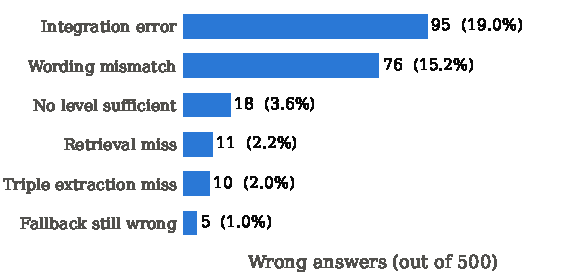
\includegraphics[width=\columnwidth]{fig_errors.pdf}
\caption{The 215 wrong answers, grouped by the stage where the error first appears.}
\label{fig:errors}
\end{figure}

Figure~\ref{fig:errors} groups the 215 wrong answers by the first stage at which each one
goes wrong. Retrieval and triple extraction together account for only 21, so evidence
gathering is not the bottleneck. Instead, the bottleneck is the integration stage, where the
model selects the core triple set. This stage alone accounts for 95. A further 76 answers
are correct in content but receive 0 on EM because their wording differs
(\S\ref{sec:setup}). This is a problem with the metric rather than the method. The next two
subsections examine the 95 integration errors.

\subsection{The stopping test fires too early}
\label{sec:limit-suf}

\begin{table}[t]
\centering\small
\begin{tabular}{lrr}
\toprule
\textbf{Configuration} & \textbf{EM} & \textbf{F1} \\
\midrule
Full cascade              & 57.00 & 73.05 \\
\midrule
\quad triples only        & 57.40 & 72.99 \\
\quad sentences only      & 60.80 & \textbf{75.38} \\
\quad passages only       & \textbf{61.20} & 75.16 \\
\quad triples + sentences & 57.00 & 73.03 \\
\quad triples + passages  & 56.80 & 72.78 \\
\midrule
\quad $L=1$               & 52.60 & 67.52 \\
\quad $L=2$               & 57.40 & 73.18 \\
\bottomrule
\end{tabular}
\caption{Ablation. Every variant keeps the fallback level from \S\ref{sec:fix}, so the rows
compare against each other but not directly against Table~3 of the original paper. The last
two rows show performance levelling off from $L{=}2$ onward.}
\label{tab:ablation}
\end{table}

The cascade provides no benefit in our setting and sometimes causes harm. Two variants that
remove it, one that always reads sentences and one that always reads passages, beat the full
cascade by 3.8 and 4.2 EM points ($p < 0.005$, McNemar). Only the triples-only variant matches
the cascade. Table~\ref{tab:ablation} therefore contrasts with Table~3 of the original paper,
where the cascade beats every single-level variant.

The cascade fails because it relies on a signal that a strong backbone does not send. The
$\mathrm{Suf}$ test permits a wider context only when the model returns the refusal string,
but Gemini 2.5 Flash rarely returns it. For 361 of the 500 questions, the system stops at the
triple level immediately. \S\ref{sec:fix} explains this mechanism and proposes a
replacement.

Table~\ref{tab:ablation} also shows that performance becomes flat from $L{=}2$ onward, so the
number of rounds is not the bottleneck.

\subsection{Every context level contains the filter's gaps}
\label{sec:limit-empty}

The second failure occurs when the system refuses to answer even though the evidence has
already been retrieved. All three levels come from the same core triple set. Thus, anything
dropped by the filter is missing from $F$, $S$ and $D$ alike, and widening the context only
presents the same gap in a longer form. The model refuses at every level, and the system
enters the default branch of Equation~\ref{eq:acmg}. This branch handles 73 questions, all
incorrect, although 66 of them have retrieval recall of 1.0. The retrieval module found
enough evidence, but the filter removed it. The group that suffers most is comparison
questions, 24 out of 51, because the filter usually keeps triples about only one of the two
entities.

\section{Replacing the Stopping Test with an Evidence Test}
\label{sec:fix}

$\mathrm{Suf}$ uses the refusal string as its signal of whether the context is sufficient,
but this signal is wrong in both directions. The model refuses when the evidence is already
present (\S\ref{sec:limit-empty}), and it answers when evidence is missing
(\S\ref{sec:limit-suf}). We address the first direction first because the gains from the two
changes are additive.

\paragraph{The model refuses although the evidence is present.} We add a final level that is
not built from the core set. When no level in the cascade produces an answer, the system
rereads all retrieved passages instead of only those indicated by the triples. This level
raises EM from 50.80 to 57.00 and reduces refusals from 73 to 35. It handles 38 questions, of which 31 are answered
correctly.

\paragraph{The model answers although the evidence is missing.} In this case, the system
stops at the triple level with an answer that reads well but is wrong, and the output gives
no warning. The model is not inventing answers. Among the 262 questions whose answers can be
string-matched, 252 contain the answer word for word in the core triple set. The model reads
the triples it receives correctly, but the triples themselves are insufficient.

We can measure which sets are sufficient by counting how many passages each set spans, read off the provenance map $M^D$ (\S\ref{sec:method}). Sets that span a single passage score
35.7 EM, while those that span two score 71.6. Every ViMQA question requires evidence from at
least two passages. A core set drawn from one passage is therefore insufficient by
construction, however willing the model is to answer.

We therefore add a test on the evidence alongside the existing test on the answer:
\begin{equation}
\label{eq:newsuf}
\mathrm{Suf}'(a, F) = \mathrm{Suf}(a) \cdot \mathbf{1}\!\left[\lvert M^D(F) \rvert \ge h\right]
\end{equation}
where $h$ is the number of documents the question requires. When the test fails, the system
skips the narrow levels and reads the widest one directly. The test only rereads information
the method already stores, so it costs no extra model calls, and $h = 2$ comes from the known
structure of the dataset rather than from tuning on the evaluation set.

\paragraph{Results.} With both changes, CIRAG moves from behind IRCoT to ahead of it
(Table~\ref{tab:main}). The new test alone adds 3.40 points, with a paired McNemar test at
$p = 0.0005$. It fixes 20 questions while breaking only 3. When we change the backbone to
Qwen3-30B-A3B, the improvement has the same direction but is smaller and not significant
(55.40 to 57.00 EM, $p = 0.12$). Notably, after the change, CIRAG leads IRCoT by exactly 1.4
points on both backbones, while it previously matched or trailed IRCoT.

\paragraph{What the change does not achieve.} It does not beat the passages-only variant in
Table~\ref{tab:ablation}: 60.40 against 61.20, with McNemar at $p = 0.56$. The remaining
benefit is lower cost, and this amounts to only 2.3\% of total input tokens because the ICI
stage, rather than the answering step, consumes most of them.

\section{Ruling Out Four Explanations}
\label{sec:ruleout}

We test each explanation below with an experiment that changes exactly one variable. The
reproduction in \S\ref{sec:results} already rules out the first explanation, a faulty
reimplementation.

For the second explanation, we wrote the Vietnamese prompts ourselves, while the English
prompts came from the authors. Prompt quality could therefore explain the gap. We rerun all
500 questions with the original prompts and add one line requiring a Vietnamese answer. The
result is 57.40 EM against 57.00, while the distribution across context levels changes very
little.

The third explanation asks whether one pipeline stage fails on the Vietnamese data. We keep
the backbone fixed and compare retrieval recall, the share of integration steps that keep at
least one triple, and the share that produce a next query. All three measures differ by less
than five points across the two datasets, so the pipeline behaves similarly in both
languages.

The fourth explanation requires a correction. If NativeRAG is the reference rather than
IRCoT, the CIRAG margin shrinks from 8.8 to 1.8 points as the backbone becomes stronger. This
can easily be read as evidence that the backbone matters. However, NativeRAG benefits
unusually strongly from a better backbone because it reads all ten passages directly. The
shrinking margin therefore reflects improvement in NativeRAG rather than decline in CIRAG.
If IRCoT is the reference, changing the backbone alters the margin by only 0.8 points,
compared with the 15.2 points caused by changing the dataset.


\paragraph{What remains.} After ruling out all four explanations, the only significant
difference is by question type. CIRAG leads IRCoT by 4.5 points on yes/no questions
($n = 156$, $p = 0.15$) but trails by 4.9 points on open-ended questions ($n = 344$,
$p = 0.031$). Open questions require the system to reproduce a specific phrase word for
word. Compressing context into triples has the greatest cost in such cases because triples
have already removed the original wording.

\section{Conclusion}
\label{sec:conclusion}

CIRAG's 14-point margin does not appear on ViMQA, and the cause lies in the method's own
stopping test. The lesson extends beyond CIRAG. A stopping test based on a model's behaviour
can be trusted only while the model continues to show that behaviour. As the backbone
becomes stronger, it refuses less often, so wider context levels remain unused without any
signal in the output. A test based on the evidence prevents this silent failure.

\section*{Limitations}

Our main conclusion rests on two datasets, and the reproduction on 2WikiMQA covers only 100
questions with a 770-passage corpus, far fewer than the 1,000 questions used in the original paper.
A smaller setting makes retrieval easier, so the reproduction only works in one direction: it
removes the suspicion of faulty code, but it does not prove the two builds are equivalent.

Ruling out the backbone rests on two models, enough to show its contribution is small next to
the dataset effect, but not enough to describe how the benefit varies with capability. Finally, the two ways EM scores 0 on a correct answer
(\S\ref{sec:setup}) affect all three methods: the 99 questions with long reference answers
alone account for 89 of CIRAG's 215 errors.

\bibliography{custom}

\end{document}
